%% Overall styling
\documentclass[10pt,titlepage]{article}
\usepackage[a5paper,margin=0.5in]{geometry}
\def\authorship{Bryant Eisenbach (bje2113)}
\def\class{ELEN E6950}

\author{\authorship}
\title{A Study in the Properties of Ad-Hoc Networks}

%% Header
\usepackage{fancyhdr,lastpage}
\usepackage[mmddyyyy]{datetime}
\renewcommand{\dateseparator}{/}
\fancypagestyle{plain}{
    \fancyhf{} %Clear Everything.
    \lhead{ \authorship }
    \chead{ \class }
    \rhead{ \jobname\ Page \thepage\ of \pageref*{LastPage} }
    \setlength{\headheight}{30pt}
    \setlength{\footskip}{24pt}
    \renewcommand{\headrulewidth}{1pt} %0pt for no rule, 2pt thicker etc...
    \renewcommand{\footrulewidth}{0pt}
}
\pagestyle{plain}


%% Font
\usepackage[sfdefault,light]{roboto}
\fontsize{11}{14}

%% URLs
\usepackage[ocgcolorlinks]{hyperref}
\urlstyle{same}
\renewcommand\UrlFont{\color{blue}}
\hypersetup{%
  colorlinks = true,
  linkcolor  = black
}

%% Titled appendices
\usepackage[titletoc,page]{appendix}

%% Bibliography
\usepackage[english]{babel}
\newcommand{\makebibliography}[1]{%
    \small
    \bibliographystyle{plain}
    \bibliography{#1}
}

%% Lists
\usepackage[shortlabels]{enumitem}
% Create environment that allows full-width text within list
\makeatletter
\newenvironment{fullwidth}
{\par%
    \setlength{\@totalleftmargin}{0pt}%
    \setlength{\linewidth}{\hsize}%
    \list{}{\setlength{\leftmargin}{0pt}}
\item\relax}
    {\endlist}
    \makeatother


%% Graphs and Tables
\usepackage{pgf}
\usepackage{tikz}
\usetikzlibrary{arrows,automata}

%% CSV Files
\usepackage{csvsimple}

%% Graphs
\usepackage[utf8]{inputenc}
\usepackage{pgfplots}
\usepackage[font={footnotesize,it}]{caption}
\usepackage{subcaption}
\usepgfplotslibrary{groupplots}
\pgfplotsset{width=10cm,compat=1.7}
\pgfplotsset{every axis legend/.append style={
                at={(0,0)},
             anchor=north east}
}

%% Helper for processing tikz graphs
\newcommand{\sidebysidefigures}[6]{
\par
\begin{figure}
    \centering
    \begin{subfigure}{.5\linewidth}
        \centering
        \resizebox{\linewidth}{0.8\linewidth}{%
            \input{#1}
        }
        \caption{#2}
    \end{subfigure}%
    \begin{subfigure}{.5\linewidth}
        \centering
        \resizebox{\linewidth}{0.8\linewidth}{%
            \input{#3}
        }
        \caption{#4}
    \end{subfigure}
    \caption{#5}
    \label{#6}
\end{figure}
\par
}

%% Tables 
\usepackage{booktabs}
\usepackage{longtable}
\usepackage{multirow}

% Non-floating Captions
\usepackage{capt-of}

%% Maths
\usepackage{amsmath}

%% Patches (because this distro has an old version of LaTeX
\usepackage{fixltx2e}


\begin{document}
    \maketitle

    \pagebreak
    \tableofcontents
    
    \pagebreak
    \section{Abstract}
    \section{Abstract}
Wireless Ad-Hoc Networks are a very active area of current research.
They have the ability to supplement or completely supplant wireless connectivity between peer devices,
especially in circumstances like protests, concerts, and other outdoor events where a large number of
unexpected wireless users need service, overwhelming traditional base stations.
This technology will allow communication between two participants irregardless of the load on the
traditional systems, and can dynamically grow and adapt to changing circumstances in order to provide
a robust conduit for communication.

However, this technology also has a myriad of issues due to managing interference,
and is particularly sensitive to the number of users available: 
too little, and the network has a hard time making connections;
too many, and the interference makes routing very difficult.
This project seeks to model the communication properties of Homogeneous Ad-Hoc networks, 
measure their effectiveness (dropped packets and messaging latency),
and provide a basis for drawing conclusions about such networks 
by simulating over a wide range of end users, 
modeled using the assumption that all devices are communicating 
using a simplified On-Demand Routing protocol implemented on homogeneous hardware.

    
    \pagebreak
    \section{Introduction and Background}
    \section{Introduction}
\subsection{Motivation}
While many poor inhabitants of developing countries now own cellular devices in 2016, the cost
of cellular network services is still prohibitive enough that many users don't use the services
provided by these networks unless absolutely necessary.
This has lead to primitive yet ingenious methods of communication devised by users to exchange 
messages with each other by placing missed calls -- which do not incur charges -- in order to 
reduce costs for themselves and their families \cite{beeping}.
However ingenious, this clearly demonstrates one scenario where reliable Ad-Hoc Networking
technologies are needed to supplement the connections of users and allow them to freely 
communicate with their friends and family over a coverage area of a small town.

Similar needs can be demonstrated when discussing communication during a protest,
where a malevolent government may disrupt regular cellular communications to a crowd of people,
or keeping in touch with a friends during a concert, where overuse of the existing 
wireless infrastructure could lead to issues that ad-hoc networking can solve and prevent or 
reduce possible emergencies in this situation.
A recent example is the app Jott \cite{jott-techcrunch,jott-forbes}, which connects it's users
using ad-hoc networking over the Wi-Fi protocol. In the interview, co-founder Jared Allgood
discusses that technologies like this will be very in-demand in the future, as cellular 
communication costs remain high but people still want to communicate with friends and family.

While the need for this technology is very apparent over a wide range of possible scenarios,
in reality there are a host of technical issues that are not well understood about the technology.
Scaleability is one area of concern that has been studied in detail \cite{lee01}, as these
technologies suffer from scaleability problems as the number of users grows larger.
However, through my search of the literature, it doesn't appear that the effects of scaleability
are studied as users get more spread out over an area such as in our first example.
Therefore, it seemed pertinent to create a simulation framework that allows simulations through
a wide variety of conditions, such that we may draw conclusions about these conditions in order
to focus development of these technologies more towards these kinds of users.

\subsection{Background}
In order to create a simulation on this scale, it was necessary to make a few assumptions
and further investigate the sorts of routing protocols developed for this purpose.
Our first assumption was to assume that all users are using homogeneous hardware and messages.
This means that we could assume that all users had the same transmission strength (or radius),
all messages could be represented simply by a reduced protocol, and that no other inconsistencies
would have to be modeled for our user model.
Secondly, we assumed that all users would be active at all times (available to send or receive
messages), there would be no dynamic delays in processing, and there were no inherent delays in
communication between any node.
Lastly, we assumed that overall communication happened randomly in short, one-message bursts,
such that overall communication of a single message could be measured simply as receipt of the
individual packets.

With the assumptions in place, we needed a transmission and routing protocol in order to produce
message routing that accurately models the communications between nodes.
Initially, the AODV algorithm \cite{perkins99,royer00} was studied for implementation into the
user-node model, however due to time constraints the algorithm was simplified to a very simple
stack-based broadcast re-transmission model where each node attempts re-transmission of any
messages it hears by storing those messages in a limited size storage stack.
If a node exceeds it's re-transmit stack, it pops the oldest message and appends the new message 
onto the stack.
The message itself stores the transmission list, so a user can avoid re-transmitting the same
message and flooding the stack.
While potentially unrealistic, this algorithm allowed the project to come up with accurate
results similar to those obtained by a real implementation of AODV \cite{morshed08}.

    
    \pagebreak
    \section{Methodology}
    \section{Methodology}
The objective of the project was to produce a parameterized simulation 
that could represent an ad-hoc networking scenario and compare the effects 
of different parameters on the overall communications system in terms of 
per-user average success rate (succssfully received messages) 
and latency of those messages.

The simulation was developed in several compontents.
The first stage of the simulation is the map creation layer,
which places N users (ceullar devices) randomly on an \textit{n x m} map at a
given (x, y) coordinate with a given starting radius (communication range).
The map creation stage can be instaniated for a new simulation dynamically, 
but additional methods exist to process files containing generated lists of 
users so that statically determined arrangements can be tried.
This layer was leveraged to create several static lists of different quantity
and arrangements of users, which were used for analysis by the main simulation.
Figure \ref{fig:usergraph} is an example userlist generated for the Intensity Ratio simulation.
Each user is modeled as a black point with the radius of the user colored in
for visualization purposes.
\par
\begin{figure}
    \begin{tikzpicture}

\begin{axis}[
xmin=-20, xmax=120,
ymin=-20, ymax=120,
axis on top
]
\addplot [only marks, scatter, scatter src=explicit, colormap={mymap}{[1pt]
  rgb(0pt)=(0,0,0.5);
  rgb(22pt)=(0,0,1);
  rgb(25pt)=(0,0,1);
  rgb(68pt)=(0,0.86,1);
  rgb(70pt)=(0,0.9,0.967741935483871);
  rgb(75pt)=(0.0806451612903226,1,0.887096774193548);
  rgb(128pt)=(0.935483870967742,1,0.0322580645161291);
  rgb(130pt)=(0.967741935483871,0.962962962962963,0);
  rgb(132pt)=(1,0.925925925925926,0);
  rgb(178pt)=(1,0.0740740740740741,0);
  rgb(182pt)=(0.909090909090909,0,0);
  rgb(200pt)=(0.5,0,0)
}, visualization depends on={\thisrow{sizedata} \as\perpointmarksize}, scatter/@pre marker code/.append style={/tikz/mark size=\perpointmarksize}]
table [x=x, y=y, meta=colordata]{%
x                      y                      colordata              sizedata
+7.459090885475142e+01 +3.539363377257585e+01 +6.685972099374399e-01 +1.000000000000000e+01
+1.072648067505945e+01 +5.237244617103784e+01 +4.798708121888173e-01 +1.000000000000000e+01
+8.161773952416821e+01 +5.811300790300644e+01 +9.894231117543170e-01 +1.000000000000000e+01
+4.834642700136421e+01 +6.401694267132378e+01 +6.211283300248572e-01 +1.000000000000000e+01
+3.041703763376190e+01 +1.092274426183900e+01 +9.214874440034894e-01 +1.000000000000000e+01
+7.617824939843777e+01 +6.924233949153952e+01 +1.337328331873407e-01 +1.000000000000000e+01
+9.012886591473981e+01 +6.834498110644745e+01 +8.505563247814649e-01 +1.000000000000000e+01
+8.999104673474069e+01 +8.719790096499403e+01 +4.180496935856070e-01 +1.000000000000000e+01
+8.949398064943543e+01 +3.635965505268689e+01 +7.732075734705480e-01 +1.000000000000000e+01
+4.065976584323990e+01 +7.795946195634635e+01 +3.407799557079070e-01 +1.000000000000000e+01
+9.753884440914430e+01 +7.361404255698994e+01 +6.574373013172986e-01 +1.000000000000000e+01
+6.732501674366254e+01 +1.110486244064456e+01 +1.994302411137353e-01 +1.000000000000000e+01
+1.314642908238736e+01 +5.802145335656703e+01 +2.235071593508359e-01 +1.000000000000000e+01
+8.704854841302708e+01 +5.247791773154085e+01 +9.172226335719869e-01 +1.000000000000000e+01
+8.210817375353699e+01 +9.342638177214066e+01 +3.317317140430129e-01 +1.000000000000000e+01
+7.670284874322209e+01 +1.797700651606122e+01 +5.358358895257488e-01 +1.000000000000000e+01
+2.072271754474474e+01 +8.105274892401192e+01 +8.626795882320477e-01 +1.000000000000000e+01
+4.438832846192208e+01 +6.948757327248122e+00 +2.500728020268650e-01 +1.000000000000000e+01
+7.739869754512634e+01 +7.838456490779974e+01 +2.398797424719341e-01 +1.000000000000000e+01
+3.270208738980129e+01 +6.986992094648002e+01 +8.512910807842052e-01 +1.000000000000000e+01
+4.567192881369905e+01 +5.531416843518837e+01 +5.113789572854077e-01 +1.000000000000000e+01
+8.074745798907432e+01 +5.278625726470998e+01 +6.441595651789217e-01 +1.000000000000000e+01
+3.800618539388456e+00 +1.898035223689788e+01 +6.604176079905619e-01 +1.000000000000000e+01
+7.144504813871809e+01 +3.936059813620913e+01 +4.218089127301572e-02 +1.000000000000000e+01
+7.396305897822700e+01 +9.761773054583462e+01 +8.212757902525076e-01 +1.000000000000000e+01
+1.270745159588615e+00 +8.064273835847224e+00 +1.627730396316432e-01 +1.000000000000000e+01
+5.323942877143768e+01 +8.340942724332746e+01 +8.031682534481044e-01 +1.000000000000000e+01
+5.369519592670735e+00 +9.562250006345330e+01 +3.870562688904696e-01 +1.000000000000000e+01
+6.154942288244847e+00 +4.173772357829102e+01 +3.867480725967365e-01 +1.000000000000000e+01
+2.925862978550109e+01 +8.631139407524968e+00 +3.574697539310046e-02 +1.000000000000000e+01
+4.277546513846524e+01 +2.860549030064020e+01 +8.095548818098083e-01 +1.000000000000000e+01
+8.322064202194335e+00 +9.220460155446591e+01 +7.914664934647173e-01 +1.000000000000000e+01
+3.165110489601886e-01 +9.715469482611766e+01 +6.257334922635519e-01 +1.000000000000000e+01
+8.463542898004346e+01 +5.424664799258552e+01 +7.962576334985538e-01 +1.000000000000000e+01
+8.641161769611119e+01 +5.426984704255544e+01 +2.286758026089172e-01 +1.000000000000000e+01
+7.355960263914938e+01 +5.349449932574424e+00 +8.132289090472478e-01 +1.000000000000000e+01
+3.754349772773659e+01 +3.282987029320351e+01 +8.458128884613919e-01 +1.000000000000000e+01
+8.218839925749361e+01 +6.192201382490909e+01 +2.760313997110988e-01 +1.000000000000000e+01
+9.675551069151030e+01 +4.212176738330419e+01 +8.410548731824899e-01 +1.000000000000000e+01
+7.505700353425038e+01 +4.668878136878691e+01 +3.154108016442078e-01 +1.000000000000000e+01
+2.312851447393848e+01 +1.936697515232211e+00 +2.173168027510437e-01 +1.000000000000000e+01
+3.945900937818263e+01 +6.826783483491251e+01 +9.584295100679692e-01 +1.000000000000000e+01
+1.673493876093390e+01 +4.324763883254897e+01 +3.101009581936455e-01 +1.000000000000000e+01
+2.484921902521985e+01 +3.169244833562890e+00 +5.452520123644984e-01 +1.000000000000000e+01
+5.266031635086029e+01 +7.467706390247297e-01 +2.297972258037179e-01 +1.000000000000000e+01
+5.304950811926778e+01 +7.224329498163958e+01 +5.446527235829153e-01 +1.000000000000000e+01
+8.929980915371722e+01 +8.789321664683559e+00 +8.441868110605634e-01 +1.000000000000000e+01
+7.563682390342728e+01 +6.581221798257452e+01 +4.210215015850803e-01 +1.000000000000000e+01
+1.146611946203677e+01 +4.643457777953001e+01 +8.636523092442028e-02 +1.000000000000000e+01
+2.743089153111639e+01 +3.839822922061242e+01 +5.337316153826164e-01 +1.000000000000000e+01
+8.725352438752533e+01 +2.675140892080330e+01 +4.275369973164085e-01 +1.000000000000000e+01
+4.405513398491767e+01 +6.578958091732331e+01 +6.619255016842206e-01 +1.000000000000000e+01
+6.583333031850593e+01 +7.461827951728662e+01 +4.794425107689720e-01 +1.000000000000000e+01
+2.372919261408384e+01 +4.519539307027510e+01 +5.929295410813413e-01 +1.000000000000000e+01
+7.410524436539805e+01 +2.643559619931185e+01 +9.627510018914293e-01 +1.000000000000000e+01
+9.146740937151144e+01 +4.299121238568523e+01 +5.782115356514119e-01 +1.000000000000000e+01
+5.947504429580608e+01 +9.443330922410807e+01 +1.235531648520408e-01 +1.000000000000000e+01
+5.305727994754640e+01 +4.465193766982800e+01 +1.609855768953745e-01 +1.000000000000000e+01
+5.404708137176709e+01 +2.293863872516334e+01 +1.139336505899891e-01 +1.000000000000000e+01
+4.671790404488846e+01 +4.838217686859174e+01 +4.028339377767198e-01 +1.000000000000000e+01
+2.851040682705223e+01 +9.034387583693015e+00 +2.104545974149497e-01 +1.000000000000000e+01
+5.722735040371067e+01 +1.082493903566848e+01 +9.955627860928884e-02 +1.000000000000000e+01
+4.543014200135944e+01 +1.695251059673819e+00 +5.888674987930420e-02 +1.000000000000000e+01
+9.807802509001029e+01 +5.600129103980949e+01 +5.761322152541913e-01 +1.000000000000000e+01
+8.475443772738603e+01 +2.615189019686553e+01 +3.580225122271710e-01 +1.000000000000000e+01
+3.017124029929794e+01 +4.709554240159954e+01 +9.147046294050275e-01 +1.000000000000000e+01
+2.621702174056087e+01 +1.567848107048908e+00 +6.164119060230921e-02 +1.000000000000000e+01
+4.359374117789365e+01 +8.200136933690175e+01 +9.058930222165679e-01 +1.000000000000000e+01
+6.572393857596504e+01 +7.820232085537589e+01 +1.403173964240205e-01 +1.000000000000000e+01
+5.192478638224611e+01 +9.596383682377268e+01 +9.680196696341239e-01 +1.000000000000000e+01
+5.236715061434669e+01 +3.920698196548478e+00 +9.236885691755949e-01 +1.000000000000000e+01
+7.910864281359142e+01 +8.994298977131629e+01 +6.267198250802942e-01 +1.000000000000000e+01
+1.147594637069317e+01 +9.051196875737256e+01 +5.783738442802011e-02 +1.000000000000000e+01
+8.706428765939478e+01 +1.018942668320667e+01 +1.114640278386124e-01 +1.000000000000000e+01
+6.160399494587533e+01 +1.606274672321383e+01 +8.421725099541121e-01 +1.000000000000000e+01
+7.757862640126535e+01 +6.219042588378608e+01 +8.804647624110871e-01 +1.000000000000000e+01
+7.122239393396418e+01 +5.569186345110288e+01 +5.365746558812284e-01 +1.000000000000000e+01
+7.120480081123996e+01 +9.379031381566595e+01 +2.292640646274660e-01 +1.000000000000000e+01
+6.293019415932374e+01 +2.983060374008699e+01 +7.956504453663424e-01 +1.000000000000000e+01
+2.998523233361318e+01 +2.865829251379111e+01 +2.637637706927377e-01 +1.000000000000000e+01
+3.850797995356847e+00 +8.540249755455901e+01 +8.350662315789855e-01 +1.000000000000000e+01
+8.807041540308487e+01 +3.099466392423209e+01 +3.383670948355719e-01 +1.000000000000000e+01
+4.113458612992207e+01 +9.837920673438860e+01 +2.508378030228012e-01 +1.000000000000000e+01
+3.821317148673150e+01 +8.996973752017681e+01 +8.213397599576071e-01 +1.000000000000000e+01
+7.313126289823762e+01 +7.408564282688064e+01 +2.639189487163796e-02 +1.000000000000000e+01
+7.283550013914660e+01 +8.890778335052207e+01 +6.527369954459536e-01 +1.000000000000000e+01
+7.931672011485927e+01 +9.841701545234723e+01 +3.247014679427226e-01 +1.000000000000000e+01
+5.235605347755700e+01 +9.108157960686437e+01 +4.700473327200674e-01 +1.000000000000000e+01
+5.407026653313798e+01 +7.526527973514798e+01 +4.213079664983114e-01 +1.000000000000000e+01
+9.803387610929305e+01 +4.130870467770843e+01 +7.639318207144506e-01 +1.000000000000000e+01
+4.217361741599767e+01 +9.293018593422953e+01 +7.837963705702670e-01 +1.000000000000000e+01
+5.210408192291168e+01 +3.814445159320468e+01 +1.200906618991215e-02 +1.000000000000000e+01
+8.882507720276091e+01 +9.533107892178081e+01 +3.078626306377292e-01 +1.000000000000000e+01
+2.079852278170107e+01 +6.701840212898479e+01 +1.263669190665240e-02 +1.000000000000000e+01
+7.297217619390560e+01 +6.262187052058514e+01 +9.561095813733824e-01 +1.000000000000000e+01
+5.720143427537271e+01 +9.402771890407749e+01 +5.472442282245766e-01 +1.000000000000000e+01
+5.132874215707817e+01 +5.686399849163885e+01 +3.300918422700292e-01 +1.000000000000000e+01
+6.580967905112645e+00 +6.163901125309989e+01 +6.242987962383173e-01 +1.000000000000000e+01
+9.547861210614357e+01 +9.514816629597819e+01 +1.085981437008798e-01 +1.000000000000000e+01
+1.013941140793581e+01 +2.013007168213992e+01 +7.973885510480649e-02 +1.000000000000000e+01
+9.087173426163231e+01 +7.747494801953870e+01 +1.806235279930180e-01 +1.000000000000000e+01
+3.607020624746586e+01 +6.742828269067657e+01 +9.220824541851672e-01 +1.000000000000000e+01
+9.622086587153277e+01 +1.329716244839011e+01 +2.599335476423219e-01 +1.000000000000000e+01
+6.024308324255655e+01 +1.435611791790303e-01 +5.172643335021938e-01 +1.000000000000000e+01
+8.820247352368149e+01 +2.654774822820783e+01 +4.380890298843174e-01 +1.000000000000000e+01
+2.179729430287628e+01 +5.197513410910555e+01 +6.162758402429764e-01 +1.000000000000000e+01
+3.623944240079797e+01 +4.990849473077168e+01 +2.006003826239193e-01 +1.000000000000000e+01
+1.480660247942894e+01 +1.816978609272435e+00 +4.428876563458933e-01 +1.000000000000000e+01
+1.206977036880065e+01 +7.647107385375442e+01 +6.234075001736420e-01 +1.000000000000000e+01
+5.493604582867830e+01 +9.436068177113258e+01 +7.193805852029853e-01 +1.000000000000000e+01
+8.194373134482559e+01 +5.160380973485592e+01 +7.077866564219958e-01 +1.000000000000000e+01
+5.857156735388570e+01 +2.388008236875597e+01 +7.496292547790101e-01 +1.000000000000000e+01
+3.368610024537699e+00 +8.212779495941214e+01 +1.302357288187436e-01 +1.000000000000000e+01
+8.597122508592413e+01 +8.166881367116143e+01 +1.980779138469522e-01 +1.000000000000000e+01
+1.758362923667312e+00 +4.092634815771879e+00 +7.813507959486232e-01 +1.000000000000000e+01
+6.512012000911582e+00 +9.810779124586388e+01 +6.117663229987776e-01 +1.000000000000000e+01
+4.645785838628610e+01 +5.169063222318141e+01 +8.998646450168740e-01 +1.000000000000000e+01
+6.681674901065038e+01 +6.099918009688587e+01 +4.186696870746108e-01 +1.000000000000000e+01
+7.465087030491385e+01 +7.932409145719599e+00 +5.061891723737593e-01 +1.000000000000000e+01
+9.700087359325920e+01 +2.596560474758053e+01 +4.597580285919176e-01 +1.000000000000000e+01
+7.651450673648564e+01 +9.073877650750524e+01 +6.128294440702259e-01 +1.000000000000000e+01
+6.150684566139567e+01 +7.752006783105070e+01 +6.417400437724174e-02 +1.000000000000000e+01
+9.574653849043506e+01 +2.514891011559138e+01 +1.264657519800743e-01 +1.000000000000000e+01
+6.342030703072656e+01 +9.614930369344094e+01 +1.135827957496407e-01 +1.000000000000000e+01
+5.409521760509549e+01 +7.345915449354668e+01 +8.641681518881147e-01 +1.000000000000000e+01
+2.201502491643398e+01 +5.663637637343355e+01 +2.361089532754828e-01 +1.000000000000000e+01
+6.462544767124983e+01 +6.035172305602583e+01 +8.270161343389343e-01 +1.000000000000000e+01
+6.057394999248588e+01 +5.771315412685237e+01 +5.106595128554677e-01 +1.000000000000000e+01
+3.800671304989471e+01 +7.073222919902936e+01 +8.838906167432402e-01 +1.000000000000000e+01
+3.532384749547237e+01 +2.682157853671909e+01 +3.936040925672729e-01 +1.000000000000000e+01
+2.579528734708152e+01 +1.664593511575584e+01 +7.792522632204935e-01 +1.000000000000000e+01
+5.677303402642558e+01 +4.342031719556114e+01 +4.453110650811438e-01 +1.000000000000000e+01
+3.877222039204145e+01 +9.179064525500809e+01 +3.147546483679468e-01 +1.000000000000000e+01
+8.250878824658326e+00 +4.573931516784695e+01 +7.492618749381471e-01 +1.000000000000000e+01
+3.093334054917970e+01 +8.510563371849264e+01 +8.565516954093311e-02 +1.000000000000000e+01
+6.204134960601026e+00 +8.443678155981772e+00 +6.704596865983899e-01 +1.000000000000000e+01
+9.413291996700042e+01 +6.124392104814707e+01 +5.664205306416742e-01 +1.000000000000000e+01
+7.593783478564514e+01 +3.918502017295950e+01 +6.790374263220605e-01 +1.000000000000000e+01
+8.729041750632331e+01 +4.542964305575401e+01 +3.706236391101343e-01 +1.000000000000000e+01
+1.842992677394889e+01 +1.043855648028923e+01 +4.945304793212525e-01 +1.000000000000000e+01
+5.804018191269322e+00 +6.756909986000295e+01 +9.218524680670850e-01 +1.000000000000000e+01
+7.092916489228340e+00 +5.556387033054001e+01 +6.815192482661730e-01 +1.000000000000000e+01
+8.343670212323575e+01 +7.404081768954674e+00 +5.044840867385008e-01 +1.000000000000000e+01
+8.052605223181974e+00 +8.111936689380890e+01 +6.638430815842630e-01 +1.000000000000000e+01
+9.903196202886345e+01 +9.384277356699133e+00 +4.491356082430378e-01 +1.000000000000000e+01
+4.570896590965635e+01 +3.109820218046596e+01 +6.765067033554027e-01 +1.000000000000000e+01
+7.557347650672563e+00 +5.977402431324604e+01 +7.695034070647101e-01 +1.000000000000000e+01
+2.656523306030011e+01 +7.898703959378834e+01 +7.392656110961309e-01 +1.000000000000000e+01
+1.586108914749978e+01 +3.942383948650046e+01 +1.033132749310683e-02 +1.000000000000000e+01
+9.100421940518732e+00 +4.635066545441613e+00 +8.800230538533926e-01 +1.000000000000000e+01
+4.307778170653441e+01 +4.553510250670586e+01 +7.975168762826715e-01 +1.000000000000000e+01
+9.616757863274227e+00 +7.438334919531330e+01 +8.709965592396278e-01 +1.000000000000000e+01
+7.265029562224775e+01 +3.010222907810620e+01 +9.258682720613137e-01 +1.000000000000000e+01
+3.107902504294012e+01 +5.279017687955212e+01 +7.023177651487452e-01 +1.000000000000000e+01
+2.040759226958603e+01 +7.060418579654349e+01 +9.529551107368488e-01 +1.000000000000000e+01
+5.814055326779213e+01 +1.253839615303524e+01 +9.572460296334709e-01 +1.000000000000000e+01
+4.454830642657104e+01 +1.822858638810698e+01 +3.729868210704262e-01 +1.000000000000000e+01
+9.948502117499852e+01 +7.475415199645964e+01 +7.929603196890149e-01 +1.000000000000000e+01
+8.673077086992922e+01 +4.329770140687202e+01 +8.917112746768528e-01 +1.000000000000000e+01
+8.775387904153543e+01 +1.380086672235901e+01 +3.114902836742900e-01 +1.000000000000000e+01
+8.984700579326464e+01 +6.438286754531108e+00 +8.549911197952380e-01 +1.000000000000000e+01
+5.532533044673393e+00 +1.777310091533960e+01 +6.072193316804175e-02 +1.000000000000000e+01
+8.171733421029397e+01 +3.584383088794102e+01 +8.737265753604265e-01 +1.000000000000000e+01
+8.682959759457482e+01 +2.123810467323237e+01 +6.592846187065085e-01 +1.000000000000000e+01
+5.268689399960113e+00 +4.116361352120831e+01 +3.516579354073125e-01 +1.000000000000000e+01
+4.159995370151570e+00 +1.144543132648426e+01 +1.821602378381981e-02 +1.000000000000000e+01
+5.033331370698413e+00 +8.916768128607931e+01 +4.134056001790173e-01 +1.000000000000000e+01
+5.899859289397153e+01 +3.059842113141757e+01 +7.839876265170730e-01 +1.000000000000000e+01
+9.008444498607780e+01 +9.250443027384546e+01 +1.799103969178105e-01 +1.000000000000000e+01
+9.046730765018492e+01 +6.968994991742560e+00 +8.753460589971135e-01 +1.000000000000000e+01
+1.632482971974070e+01 +5.556714820699867e+01 +3.387011538455076e-02 +1.000000000000000e+01
+8.455008741931502e-01 +1.183457444290238e+01 +7.294583250979670e-01 +1.000000000000000e+01
+7.926347696687712e+01 +9.140659748396513e+01 +2.250185952900868e-01 +1.000000000000000e+01
+2.359856258219952e+01 +4.112296877537342e+01 +6.040529698473094e-01 +1.000000000000000e+01
+8.811046366838360e+01 +7.937988770321795e+01 +9.100780728038351e-01 +1.000000000000000e+01
+7.258474561124527e+01 +6.542779314499903e+01 +1.036796636131921e-01 +1.000000000000000e+01
+7.429130625742468e+01 +8.061045537541304e+01 +8.933898590395862e-01 +1.000000000000000e+01
+4.523545806435965e+01 +8.534581250989082e+01 +5.465169346624772e-01 +1.000000000000000e+01
+2.396338327293702e+01 +6.894188462779893e-01 +4.914183212635037e-01 +1.000000000000000e+01
+8.196391685459649e+01 +2.221859407287259e+01 +1.255413114866409e-01 +1.000000000000000e+01
+5.320527127049185e+01 +5.716683613610348e+01 +2.086457421951077e-01 +1.000000000000000e+01
+4.815062689649929e-01 +5.133946237659998e+01 +5.943992970411992e-01 +1.000000000000000e+01
+2.256905766152508e+01 +8.782609968240450e+01 +9.053047896169728e-01 +1.000000000000000e+01
+9.911060649170091e+01 +2.104633898344873e+01 +9.440873975988913e-01 +1.000000000000000e+01
+1.595062711896409e+01 +9.056337611127668e+01 +6.432818815086049e-01 +1.000000000000000e+01
+9.086129772473225e+01 +9.066743843847992e+01 +1.476861226100923e-01 +1.000000000000000e+01
+5.777840340781819e+01 +5.548631158641657e+01 +2.994361172685142e-01 +1.000000000000000e+01
+9.229699977516601e+01 +5.738491987060179e+00 +1.730921128418241e-01 +1.000000000000000e+01
+8.939633262456015e+01 +6.461282587925416e+01 +7.389211628534655e-01 +1.000000000000000e+01
+8.075130019463877e+01 +6.432771209983235e+00 +9.954088947494172e-01 +1.000000000000000e+01
+6.374408786673652e+01 +1.762680989371956e+01 +1.239578942034140e-01 +1.000000000000000e+01
+9.925999863109524e+00 +8.579115248996982e+01 +7.465778033341131e-02 +1.000000000000000e+01
+9.260849192584708e+01 +2.650805439570959e+01 +8.949415896662594e-01 +1.000000000000000e+01
+8.405900549379132e+01 +8.866754648374462e+01 +6.350461040407924e-01 +1.000000000000000e+01
+6.403396481426142e+01 +7.685340872643881e+01 +7.240477422232607e-01 +1.000000000000000e+01
+1.922027135695925e+00 +1.655474457729900e+01 +5.395570522007921e-01 +1.000000000000000e+01
+1.414336199854279e+01 +8.319151262311733e+01 +8.916793049978626e-01 +1.000000000000000e+01
+8.763140763247125e+01 +5.572020039780769e+01 +2.766960524550772e-01 +1.000000000000000e+01
+4.267724611056355e+01 +4.294845060565535e+01 +6.024288095637429e-01 +1.000000000000000e+01
+5.908274588538549e+01 +9.513757133627234e+01 +6.466389113334630e-01 +1.000000000000000e+01
};
\addplot [only marks, draw=black, fill=black, colormap={mymap}{[1pt]
  rgb(0pt)=(0,0,0.5);
  rgb(22pt)=(0,0,1);
  rgb(25pt)=(0,0,1);
  rgb(68pt)=(0,0.86,1);
  rgb(70pt)=(0,0.9,0.967741935483871);
  rgb(75pt)=(0.0806451612903226,1,0.887096774193548);
  rgb(128pt)=(0.935483870967742,1,0.0322580645161291);
  rgb(130pt)=(0.967741935483871,0.962962962962963,0);
  rgb(132pt)=(1,0.925925925925926,0);
  rgb(178pt)=(1,0.0740740740740741,0);
  rgb(182pt)=(0.909090909090909,0,0);
  rgb(200pt)=(0.5,0,0)
}]
table {%
x                      y
+7.459090885475142e+01 +3.539363377257585e+01
+1.072648067505945e+01 +5.237244617103784e+01
+8.161773952416821e+01 +5.811300790300644e+01
+4.834642700136421e+01 +6.401694267132378e+01
+3.041703763376190e+01 +1.092274426183900e+01
+7.617824939843777e+01 +6.924233949153952e+01
+9.012886591473981e+01 +6.834498110644745e+01
+8.999104673474069e+01 +8.719790096499403e+01
+8.949398064943543e+01 +3.635965505268689e+01
+4.065976584323990e+01 +7.795946195634635e+01
+9.753884440914430e+01 +7.361404255698994e+01
+6.732501674366254e+01 +1.110486244064456e+01
+1.314642908238736e+01 +5.802145335656703e+01
+8.704854841302708e+01 +5.247791773154085e+01
+8.210817375353699e+01 +9.342638177214066e+01
+7.670284874322209e+01 +1.797700651606122e+01
+2.072271754474474e+01 +8.105274892401192e+01
+4.438832846192208e+01 +6.948757327248122e+00
+7.739869754512634e+01 +7.838456490779974e+01
+3.270208738980129e+01 +6.986992094648002e+01
+4.567192881369905e+01 +5.531416843518837e+01
+8.074745798907432e+01 +5.278625726470998e+01
+3.800618539388456e+00 +1.898035223689788e+01
+7.144504813871809e+01 +3.936059813620913e+01
+7.396305897822700e+01 +9.761773054583462e+01
+1.270745159588615e+00 +8.064273835847224e+00
+5.323942877143768e+01 +8.340942724332746e+01
+5.369519592670735e+00 +9.562250006345330e+01
+6.154942288244847e+00 +4.173772357829102e+01
+2.925862978550109e+01 +8.631139407524968e+00
+4.277546513846524e+01 +2.860549030064020e+01
+8.322064202194335e+00 +9.220460155446591e+01
+3.165110489601886e-01 +9.715469482611766e+01
+8.463542898004346e+01 +5.424664799258552e+01
+8.641161769611119e+01 +5.426984704255544e+01
+7.355960263914938e+01 +5.349449932574424e+00
+3.754349772773659e+01 +3.282987029320351e+01
+8.218839925749361e+01 +6.192201382490909e+01
+9.675551069151030e+01 +4.212176738330419e+01
+7.505700353425038e+01 +4.668878136878691e+01
+2.312851447393848e+01 +1.936697515232211e+00
+3.945900937818263e+01 +6.826783483491251e+01
+1.673493876093390e+01 +4.324763883254897e+01
+2.484921902521985e+01 +3.169244833562890e+00
+5.266031635086029e+01 +7.467706390247297e-01
+5.304950811926778e+01 +7.224329498163958e+01
+8.929980915371722e+01 +8.789321664683559e+00
+7.563682390342728e+01 +6.581221798257452e+01
+1.146611946203677e+01 +4.643457777953001e+01
+2.743089153111639e+01 +3.839822922061242e+01
+8.725352438752533e+01 +2.675140892080330e+01
+4.405513398491767e+01 +6.578958091732331e+01
+6.583333031850593e+01 +7.461827951728662e+01
+2.372919261408384e+01 +4.519539307027510e+01
+7.410524436539805e+01 +2.643559619931185e+01
+9.146740937151144e+01 +4.299121238568523e+01
+5.947504429580608e+01 +9.443330922410807e+01
+5.305727994754640e+01 +4.465193766982800e+01
+5.404708137176709e+01 +2.293863872516334e+01
+4.671790404488846e+01 +4.838217686859174e+01
+2.851040682705223e+01 +9.034387583693015e+00
+5.722735040371067e+01 +1.082493903566848e+01
+4.543014200135944e+01 +1.695251059673819e+00
+9.807802509001029e+01 +5.600129103980949e+01
+8.475443772738603e+01 +2.615189019686553e+01
+3.017124029929794e+01 +4.709554240159954e+01
+2.621702174056087e+01 +1.567848107048908e+00
+4.359374117789365e+01 +8.200136933690175e+01
+6.572393857596504e+01 +7.820232085537589e+01
+5.192478638224611e+01 +9.596383682377268e+01
+5.236715061434669e+01 +3.920698196548478e+00
+7.910864281359142e+01 +8.994298977131629e+01
+1.147594637069317e+01 +9.051196875737256e+01
+8.706428765939478e+01 +1.018942668320667e+01
+6.160399494587533e+01 +1.606274672321383e+01
+7.757862640126535e+01 +6.219042588378608e+01
+7.122239393396418e+01 +5.569186345110288e+01
+7.120480081123996e+01 +9.379031381566595e+01
+6.293019415932374e+01 +2.983060374008699e+01
+2.998523233361318e+01 +2.865829251379111e+01
+3.850797995356847e+00 +8.540249755455901e+01
+8.807041540308487e+01 +3.099466392423209e+01
+4.113458612992207e+01 +9.837920673438860e+01
+3.821317148673150e+01 +8.996973752017681e+01
+7.313126289823762e+01 +7.408564282688064e+01
+7.283550013914660e+01 +8.890778335052207e+01
+7.931672011485927e+01 +9.841701545234723e+01
+5.235605347755700e+01 +9.108157960686437e+01
+5.407026653313798e+01 +7.526527973514798e+01
+9.803387610929305e+01 +4.130870467770843e+01
+4.217361741599767e+01 +9.293018593422953e+01
+5.210408192291168e+01 +3.814445159320468e+01
+8.882507720276091e+01 +9.533107892178081e+01
+2.079852278170107e+01 +6.701840212898479e+01
+7.297217619390560e+01 +6.262187052058514e+01
+5.720143427537271e+01 +9.402771890407749e+01
+5.132874215707817e+01 +5.686399849163885e+01
+6.580967905112645e+00 +6.163901125309989e+01
+9.547861210614357e+01 +9.514816629597819e+01
+1.013941140793581e+01 +2.013007168213992e+01
+9.087173426163231e+01 +7.747494801953870e+01
+3.607020624746586e+01 +6.742828269067657e+01
+9.622086587153277e+01 +1.329716244839011e+01
+6.024308324255655e+01 +1.435611791790303e-01
+8.820247352368149e+01 +2.654774822820783e+01
+2.179729430287628e+01 +5.197513410910555e+01
+3.623944240079797e+01 +4.990849473077168e+01
+1.480660247942894e+01 +1.816978609272435e+00
+1.206977036880065e+01 +7.647107385375442e+01
+5.493604582867830e+01 +9.436068177113258e+01
+8.194373134482559e+01 +5.160380973485592e+01
+5.857156735388570e+01 +2.388008236875597e+01
+3.368610024537699e+00 +8.212779495941214e+01
+8.597122508592413e+01 +8.166881367116143e+01
+1.758362923667312e+00 +4.092634815771879e+00
+6.512012000911582e+00 +9.810779124586388e+01
+4.645785838628610e+01 +5.169063222318141e+01
+6.681674901065038e+01 +6.099918009688587e+01
+7.465087030491385e+01 +7.932409145719599e+00
+9.700087359325920e+01 +2.596560474758053e+01
+7.651450673648564e+01 +9.073877650750524e+01
+6.150684566139567e+01 +7.752006783105070e+01
+9.574653849043506e+01 +2.514891011559138e+01
+6.342030703072656e+01 +9.614930369344094e+01
+5.409521760509549e+01 +7.345915449354668e+01
+2.201502491643398e+01 +5.663637637343355e+01
+6.462544767124983e+01 +6.035172305602583e+01
+6.057394999248588e+01 +5.771315412685237e+01
+3.800671304989471e+01 +7.073222919902936e+01
+3.532384749547237e+01 +2.682157853671909e+01
+2.579528734708152e+01 +1.664593511575584e+01
+5.677303402642558e+01 +4.342031719556114e+01
+3.877222039204145e+01 +9.179064525500809e+01
+8.250878824658326e+00 +4.573931516784695e+01
+3.093334054917970e+01 +8.510563371849264e+01
+6.204134960601026e+00 +8.443678155981772e+00
+9.413291996700042e+01 +6.124392104814707e+01
+7.593783478564514e+01 +3.918502017295950e+01
+8.729041750632331e+01 +4.542964305575401e+01
+1.842992677394889e+01 +1.043855648028923e+01
+5.804018191269322e+00 +6.756909986000295e+01
+7.092916489228340e+00 +5.556387033054001e+01
+8.343670212323575e+01 +7.404081768954674e+00
+8.052605223181974e+00 +8.111936689380890e+01
+9.903196202886345e+01 +9.384277356699133e+00
+4.570896590965635e+01 +3.109820218046596e+01
+7.557347650672563e+00 +5.977402431324604e+01
+2.656523306030011e+01 +7.898703959378834e+01
+1.586108914749978e+01 +3.942383948650046e+01
+9.100421940518732e+00 +4.635066545441613e+00
+4.307778170653441e+01 +4.553510250670586e+01
+9.616757863274227e+00 +7.438334919531330e+01
+7.265029562224775e+01 +3.010222907810620e+01
+3.107902504294012e+01 +5.279017687955212e+01
+2.040759226958603e+01 +7.060418579654349e+01
+5.814055326779213e+01 +1.253839615303524e+01
+4.454830642657104e+01 +1.822858638810698e+01
+9.948502117499852e+01 +7.475415199645964e+01
+8.673077086992922e+01 +4.329770140687202e+01
+8.775387904153543e+01 +1.380086672235901e+01
+8.984700579326464e+01 +6.438286754531108e+00
+5.532533044673393e+00 +1.777310091533960e+01
+8.171733421029397e+01 +3.584383088794102e+01
+8.682959759457482e+01 +2.123810467323237e+01
+5.268689399960113e+00 +4.116361352120831e+01
+4.159995370151570e+00 +1.144543132648426e+01
+5.033331370698413e+00 +8.916768128607931e+01
+5.899859289397153e+01 +3.059842113141757e+01
+9.008444498607780e+01 +9.250443027384546e+01
+9.046730765018492e+01 +6.968994991742560e+00
+1.632482971974070e+01 +5.556714820699867e+01
+8.455008741931502e-01 +1.183457444290238e+01
+7.926347696687712e+01 +9.140659748396513e+01
+2.359856258219952e+01 +4.112296877537342e+01
+8.811046366838360e+01 +7.937988770321795e+01
+7.258474561124527e+01 +6.542779314499903e+01
+7.429130625742468e+01 +8.061045537541304e+01
+4.523545806435965e+01 +8.534581250989082e+01
+2.396338327293702e+01 +6.894188462779893e-01
+8.196391685459649e+01 +2.221859407287259e+01
+5.320527127049185e+01 +5.716683613610348e+01
+4.815062689649929e-01 +5.133946237659998e+01
+2.256905766152508e+01 +8.782609968240450e+01
+9.911060649170091e+01 +2.104633898344873e+01
+1.595062711896409e+01 +9.056337611127668e+01
+9.086129772473225e+01 +9.066743843847992e+01
+5.777840340781819e+01 +5.548631158641657e+01
+9.229699977516601e+01 +5.738491987060179e+00
+8.939633262456015e+01 +6.461282587925416e+01
+8.075130019463877e+01 +6.432771209983235e+00
+6.374408786673652e+01 +1.762680989371956e+01
+9.925999863109524e+00 +8.579115248996982e+01
+9.260849192584708e+01 +2.650805439570959e+01
+8.405900549379132e+01 +8.866754648374462e+01
+6.403396481426142e+01 +7.685340872643881e+01
+1.922027135695925e+00 +1.655474457729900e+01
+1.414336199854279e+01 +8.319151262311733e+01
+8.763140763247125e+01 +5.572020039780769e+01
+4.267724611056355e+01 +4.294845060565535e+01
+5.908274588538549e+01 +9.513757133627234e+01
};
\end{axis}

\end{tikzpicture}

    \caption{User graph for 100 Users Randomly placed on a 100x100 grid}
    \label{fig:usergraph}
\end{figure}
\par

The second stage was the main simulation.
This stage took a list of users, as described previously, as well as additional
parameters describing the nature of communication amoung the users such as
the intensity ratio and the number of steps (as an analogue for time) to run 
the simulation for.
At each stage of the simulation, a randomly chosen subset of all users on the map
were chosen based upon the intensity ratio to attempt to send a message to another
randomly chosen user on the map.
After the number of steps specified was reached, the simulation would continue
to allow all users to complete their retransmission queues, which would usually
take a few extra steps to complete.
Once all users had finished their retransmissions, statistics would be compiled
on a per-user basis, and overall averages would be returned.

The main simulation stage was composed of several smaller elements modeling
the messages and user interactions.
These elements were modeled relatively simplisitically, so future additions could be
made to model other complex aspects of communication e.g. multi-packet messages,
fluctuating communication range, power usage, etc.

Finally, the last stage was a statistical analysis layer which enabled taking overall
statistics over a range of parameter values and creating relevant tables and graphs,
which are used in the results portion of this paper.

The language chosen to implement the simulation was Python, due to it's incorporation of 
object-oriented paradigms, as well as the ease of prototyping a larger program in a 
short period of time.
Additionally, the author's knowledge and existance of several data tools made it a natural
fit for this project.
A full listing of all the code created for this simulation is in Appendix \ref{appendix:code}.

    
    \pagebreak
    \section{Results and Discussion}
    \section{Results and Discussion}
The simulation was run for independent variations of four parameters under constant conditions.
The constant conditions used as the baseline for the experiment are described in 
Figure \ref{fig:consttable}.
The ranges over which all the parameters were individually varied are listed in 
Figure \ref{fig:rangetable}.

\begin{figure}[!htb]
    \centering
    \begin{tabular}{l|rl}
        \hline
        Parameter               & Value     & Units                     \\
        \hline
        Grid Area               & 100x100   & feet squared              \\
        Transmission Radius     & 10        & feet                      \\
        User Population         & 200       & users                     \\
        \hline
        Intensity Ratio         & 0.05      & msgs per user per step    \\
        Simulation Duration     & 50        & steps                     \\
        \hline
    \end{tabular}
    \caption{Table of constants}
    \label{fig:consttable}
\end{figure}

\begin{figure}[!htb]
    \centering
    \begin{tabular}{l|rr}
        \hline
        Parameter               & Min   & Max       \\
        \hline
        Grid Area               & 10x10 & 160x160   \\
        Transmission Radius     & 10    & 160       \\
        User Population         & 100   & 1600      \\
        \hline
        Intensity Ratio         & 0.010 & 0.100     \\
        \hline
    \end{tabular}
    \caption{Parameter Ranges}
    \label{fig:rangetable}
\end{figure}

\subsection{User Area Separation Variation}
Figure \ref{fig:vararea} shows the results when the area is increased
(also increasing average user separation).

\sidebysidefigures
{vararea-success-rate-graph.tex}       {Success Rate vs. Area}
{vararea-average-latency-graph.tex}    {Average Latency vs. Area}
{Network Properties with Increasing Area given Constant Radius and Number of Users}
{fig:vararea}

Figure \ref{fig:vararea}a shows a exponential decay in successfully received packets.
The decay starts from near 100\% corresponding to the point where the users are crowded very close
together (user transmission radius approximately equal to grid size) and swiftly decays as
the grid size is increased.
This result means that as separation distance increases for a small population, there
is a corresponding drop-off in performance that quickly makes this kind of network non-viable.
In practice, this would mean that connecting users would need to increase their transmission radius
and therefore their power in order to overcome this limitation.
However, as cellular devices are small, this solution has limited effect.

Figure \ref{fig:vararea}b shows a logarithmic increase in latency.
The results become very erratic when the area is very large because so few messages
are received at that point.
The effect tails off as user separation increases because, even though the probability
of success is greatly reduced, the successful paths that can be formed between users
occur when communication is traveling between closely placed users in the communication path.
This increase in area shares the largest possible latencies overall as when a message does
successful travel to it's intended recipient, it has been re-transmitted by participating
users many times.
There is an artificial limit to this latency in the fact that each message has a Time-To-Live (TTL)
parameter which controls how many hops it can make before it is discarded.
In areas where user separation far outpaces transmission radius, the intuition here is to
increase the TTL message parameter to ensure a greater success rate.

\subsection{User Transmission Radius Variation}
Figure \ref{fig:varradius} shows the results when the user transmission radius is increased.

\sidebysidefigures
{varradius-success-rate-graph.tex}     {Success Rate vs. Radius}
{varradius-average-latency-graph.tex}  {Average Latency vs. Radius}
{Network Properties with Increasing Radius Area given Constant Area and Number of Users}
{fig:varradius}

Figure \ref{fig:varradius}a shows a logarithmic increase in successfully received packets.
The success rate increases from close to 0\% near the trivial case when user radius is far smaller
than the user density can support, to complete success again past the region where
the transmission radius approximately equals grid size (optimal user density).
The intuition here mirrors the intuition for the increasing grid size and produces a strong
correlation towards increasing the transmission radius (at the expense of cellular battery life)
when the user density does not support normal communication.

Figure \ref{fig:varradius}b shows a exponential decay in in latency.
There is an asymptote that is reached near the point where user transmission radius is
close to the same region where separation distance and transmission radius are approximately
equal. This asymptote could appear due to interference between transmissions as the radius 
gets larger. The intuition here is that there is an upper limit to the effectiveness of increasing
the user transmission radius based on the population size and separation distance of the users.

\subsection{User Population Variation}
Figure \ref{fig:varusers} shows the results when the user population is increased.

\sidebysidefigures
{varusers-success-rate-graph.tex}      {Success Rate vs. Number of Users}
{varusers-average-latency-graph.tex}   {Average Latency vs. Number of Users}
{Network Properties with Increasing Number of Users given Constant Area and Radius}
{fig:varusers}

Figure \ref{fig:varusers}a shows an exponential decrease in successfully received packets with
an asymptote. The asymptote appears to start around 500 users, and experiences a much gradual
linear decay after that. The point where the asymptote starts corresponds to the same saturation 
point in user density as mentioned prior. The intuition here would point to
a ceiling on the capacity that such a system can support. This could be an artificial limit based
on the size of the re-transmit stack allocated to each user device as well as the TTL of each message.
If the stack where increased, more messages could be re-transmitted potentially increasing the
likelihood of success. However, as the number of users increase the amount of interference and
capacity considerations might limit the effectiveness of such a solution. Increasing the TTL
parameter would be a better solution to increasing the success rate since a message would
logically need more hops to make it to it's destination when the area is more crowded.
This solution would also increase the overall amount of transmissions, so a trade would need to be
made in order to avoid reduced returns.

Figure \ref{fig:varusers}b shows a exponential decrease in latency. The intuition here, when coupled
with the success rate, suggests that the successful messages are between two users that are 
increasingly closer to each other as the space gets more crowded. Increasing the TTL to gain a higher
success rate would have the effect of increasing the average latency of successful messages, as
again more hops would be needed to reach destinations as the user density increases.

\subsection{Messaging Intensity Ratio Variation}
Figure \ref{fig:varintensity} shows the results when the transmission intensity ratio is increased.
Note this is the only parameter that was modeled in simulation based on the overall user population, 
instead of characteristics about the individual users.

\sidebysidefigures
{varintensity-success-rate-graph.tex}      {Success Rate vs. Intensity Ratio}
{varintensity-average-latency-graph.tex}   {Average Latency vs. Intensity Ratio}
{Network Properties with Increasing Intensity Ratio given Constant Area, Radius and Users}
{fig:varintensity}

Figure \ref{fig:varintensity}a shows a semi-linear decrease in successfully received packets.
The increase in intensity corresponds to a sharp and then gradual decrease in the rate of success.
The initial sharp decrease corresponds to the area before saturating the same threshold of
user density. However, the intuition
for the more gradual decrease after that point suggests that as the intensity increases, there
is a higher likelihood that the messaging is occurring between users that are closer together.
This corresponds to figure \ref{fig:varintensity}b, which shows a steep linear decrease in latency.
Reviewing these two graphs in parallel suggests this intuition is correct, in that an increase
in the amount of communication overall increases the load on the system, and reduces the effective
range of messaging between two users. Similar to the user density increase, the solution here
would be to increase the TTL of the messaging. However, with this increase in the liveness of
individual messages coupled with the overall increase in the number of messages, there may exist
a structural limit in the capacity of this system to deliver messages even with the increased 
liveness due because of interference.

    
    \pagebreak
    \section{Conclusion}
    \section{Conclusion}
In conclusion, we have summarized in our results some intuition to the behavior of Ad-Hoc Networks
over a variety of different situations.
We have described what the overall trend is in terms of latency and successful transmission rate
over varying area, transmission radius, and user population, as well as messaging intensity.
All of this analysis was done under the assumptions of a re-transmission algorithm
utilizing a fixed-size stack and a messaging strategy that used a static TTL parameter
that allowed for simplified modeling the communication strategies these devices typically use.
Using the intuition we have built, we can make overall recommendations that
active management of parameters such as stack size, user transmission radius/power
(and consequently user battery life), and TTL of the messages would increase the likelihood of 
success and manage a reasonable level of average latency.

%Future work
While this simulation is a good baseline for categorizing Ad-Hoc Networks, the project could
benefit from more realistic modeling of the style of communication, including more sophisticated
models for message size, messaging dynamics, power usage, and interference.
As it stands, this simulation may be an overly liberal estimate of system behavior and additional
modeling may yield to large differences in the parameters measured here.
However, this simulation provides a good backbone for those activities and hopefully future
projects may explore different possibilities in order to maximize per-user performance of
an Ad-Hoc messaging system.


    \pagebreak
    \appendix
    \renewcommand{\thesection}{\Alph{section}}
    \section{Source Code Listings}
\label{appendix:code}

\subsection{Main Simulation Source Code}
\simcode
{simulation.py: Main function}
{../simulation/simulation.py}{code:simulation.py}

\simcode
{userlist.py: Utility for creating and processing List of Users}
{../simulation/userlist.py}{code:userlist.py}

\simcode
{userregistry.py: Parent class for managing groups of users}
{../simulation/userregistry.py}{code:userregistry.py}

\simcode
{user.py: Cellular Device User class}
{../simulation/user.py}{code:user.py}

\simcode
{message.py: Messaging class}
{../simulation/message.py}{code:message.py}

\subsection{Sublemental Files}
\simcode
{argLimitedFloat.py: Utility for managing input arguments with a given range}
{../simulation/argLimitedFloat.py}{code:argLimitedFloat.py}

\simcode
{eprint.py: Helper for printing to stderr}
{../simulation/eprint.py}{code:eprint.py}

\simcode
{point.py: Helper for location processing}
{../simulation/point.py}{code:point.py}

    
    \pagebreak
    \small
    \bibliography{bibliography.bib}{}
    \bibliographystyle{plain}

\end{document}
